\section{Final shared pressure--speciation refinement}

\subsection{Question and method}

Can one small parameter block improve pressure and direct speciation together
after fixing the selected shell-Born, ion-suppressed-permittivity, and
CO$_2$--water induced-association structure? The calculation fits one common
$k_{\mathrm{CO_2,MEA}}$, $\sigma_{\mathrm{MEAH^+}}$, and
$\sigma_{\mathrm{MEACOO^-}}$ across all retained states. Each state is a
fixed-temperature, fixed-pressure, one-liquid GREPE problem. Molecular-CO$_2$
liquid fugacity supplies the fast pressure surrogate; direct Jakobsen species
mole fractions supply the speciation observations. Natural-log residuals are
normalized so pressure and speciation have equal block weight.

The installed non-editable Engine wheel has SHA-256:
\begin{center}
\small\ttfamily
e14288867d4fb5bc1367dd0de490aeb\allowbreak\\
1551f1613074aced0a8d28432ca762f23
\end{center}
The primary application domain is 30 wt\% MEA at 313.15, 333.15, and
353.15 K. All 59 available pressure observations in those profiles were
attempted. Thirty-eight pressure rows and 17 speciation targets from three
loading states entered the fit. Twenty-one pressure states and three
speciation states failed trace-state certification before the fit and remain
explicit failures rather than penalty residuals.

\subsection{Result}

\begin{table}[htbp]
\centering
\caption{Shared parameter refinement. None of the fitted values contacts its
bound.}
\begin{tabular}{lrrr}
\toprule
Parameter & Start & Fitted & Bounds \\
\midrule
$k_{\mathrm{CO_2,MEA}}$ & 0 & -0.03182703 & $[-1,1]$ \\
$\sigma_{\mathrm{MEAH^+}}$ (\si{\angstrom}) & 3.48508557 & 2.68378739 & $[1.5,5.8]$ \\
$\sigma_{\mathrm{MEACOO^-}}$ (\si{\angstrom}) & 3.53543526 & 3.26931496 & $[1.5,5.8]$ \\
\bottomrule
\end{tabular}
\end{table}

The complete-row one-step refinement reduced equal-block cost by 42.2\%, from
$0.9452311$ to $0.5460640$, in 213 seconds. This is a usable refinement, not a
formal optimizer convergence claim. Pressure-surrogate RMS and median factors
are 2.114 and 2.046; speciation RMS and median factors are 2.073 and 1.540.
Scaled-Jacobian singular values are 2.3285, 1.9298, and 0.03822; the condition
number is 60.9. No parameter contacts a bound.

\begin{figure}[htbp]
\centering
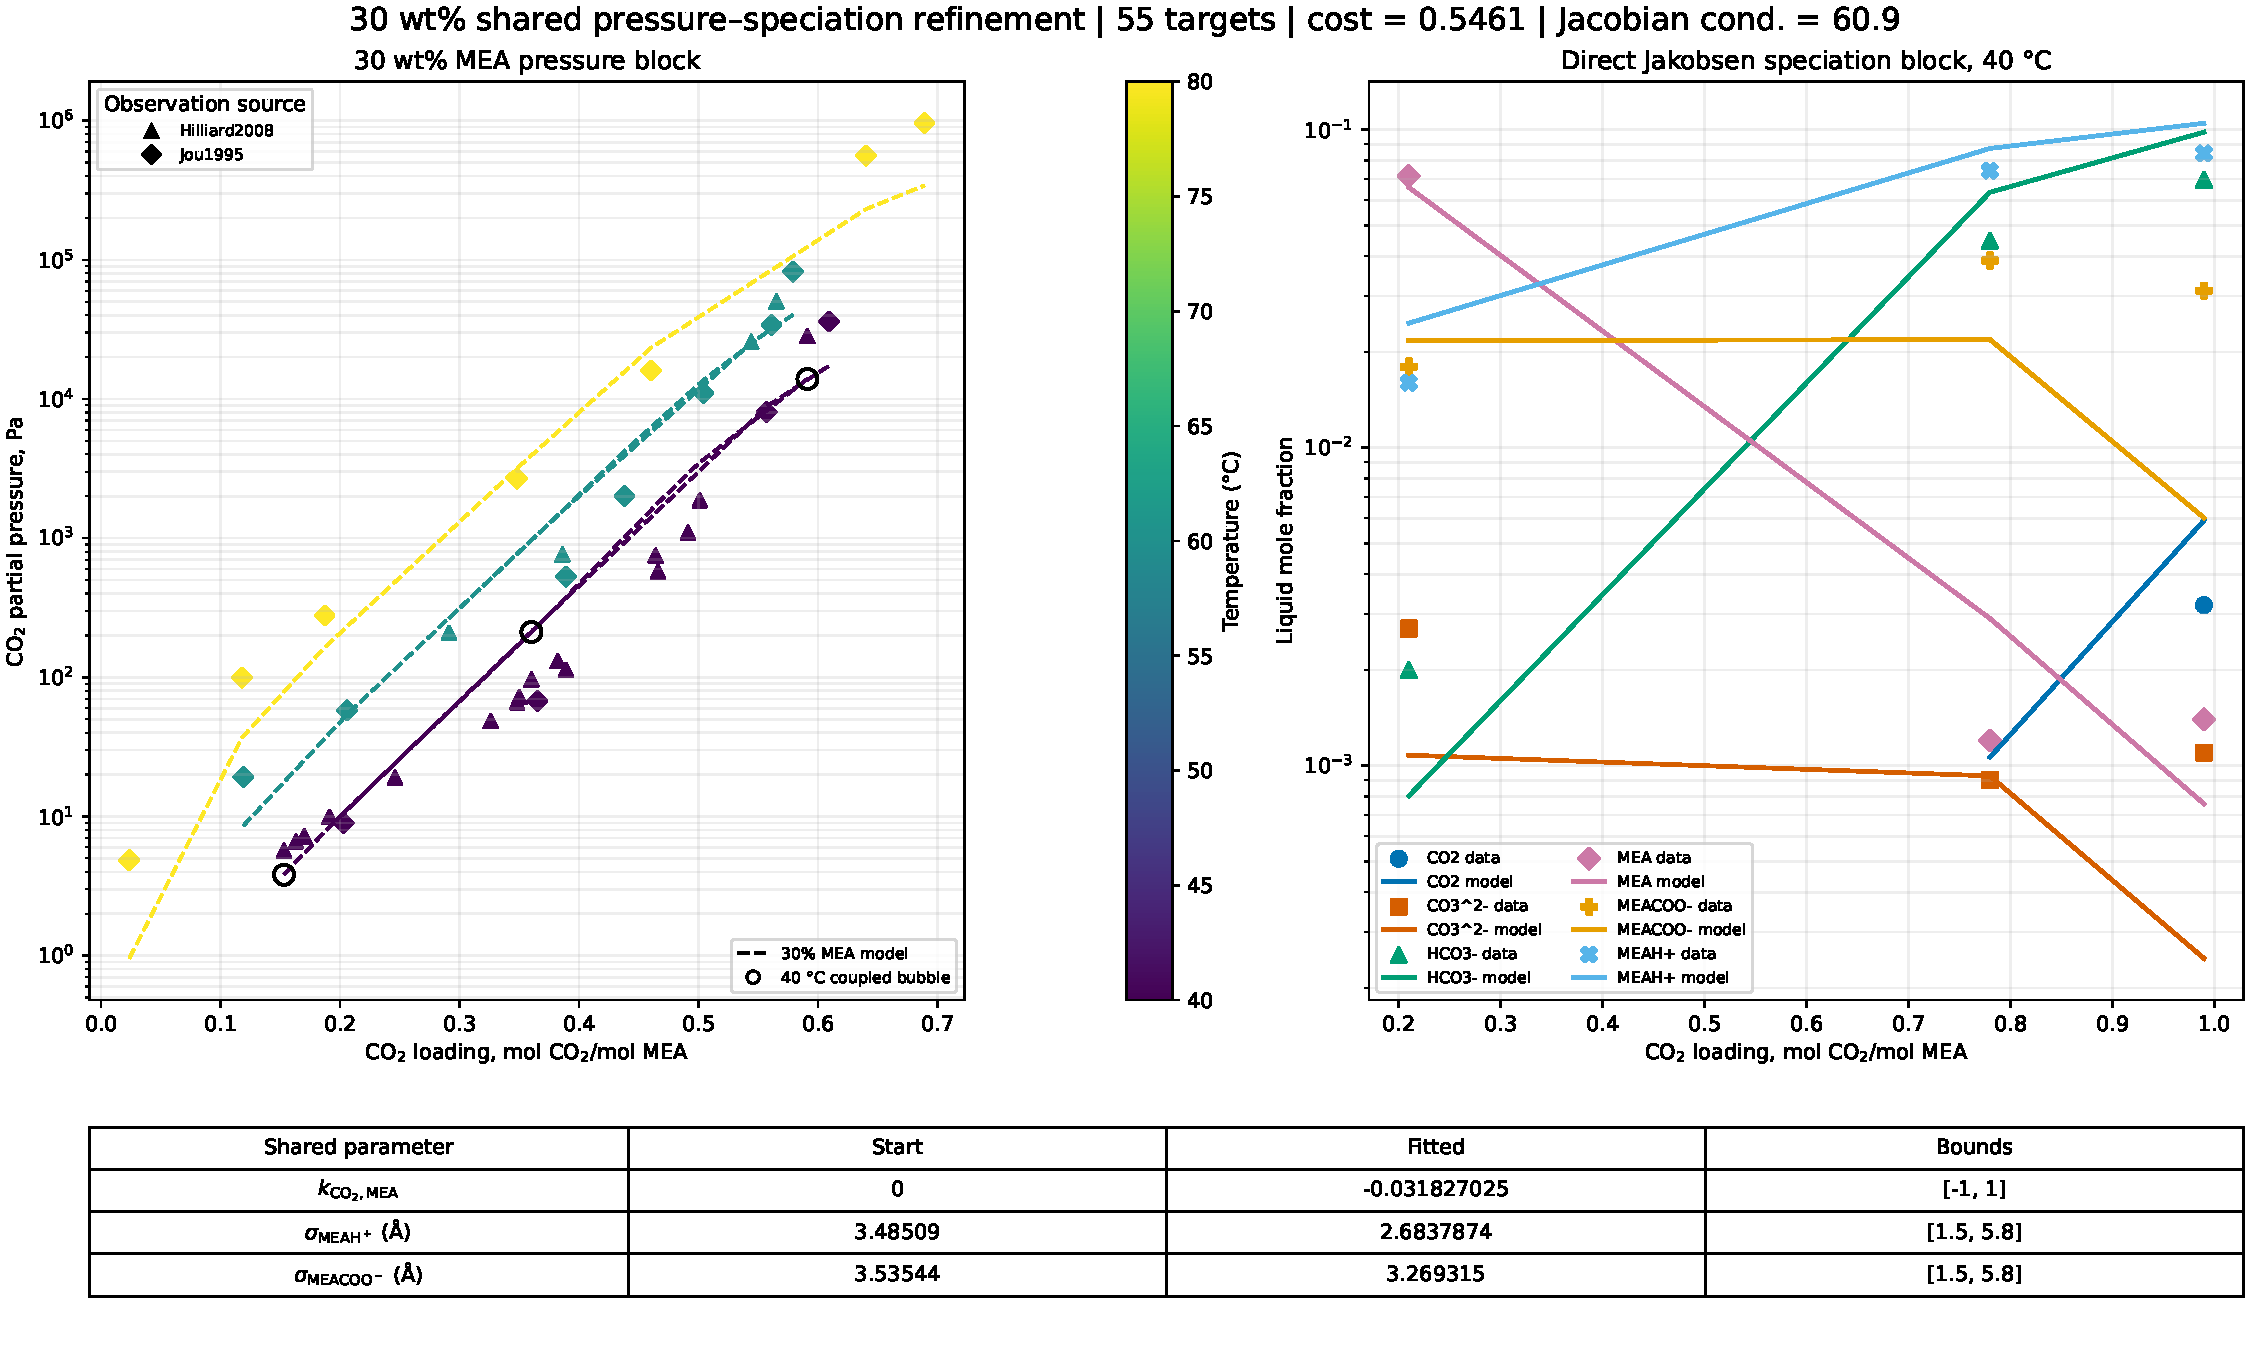
\includegraphics[width=\textwidth]{analyses/phase3/ionic_epcsaft_regression/born_permittivity_sensitivity/figures/final_shared_pressure_speciation_refinement.pdf}
\caption{Shared-parameter fit. Points are observations, lines are the
fixed-TP pressure surrogate or speciation predictions, and open circles are
independent coupled-bubble results at \SI{40}{\celsius}. The exact plotted
values are retained beside the fit result.}
\end{figure}

\subsection{Coupled phase-equilibrium check and interpretation}

Three Hilliard states at \SI{40}{\celsius} were recomputed with the declared
finite liquid and incipient vapor phases. All passed the numerical and
physical certification criteria. Predicted CO$_2$ partial pressures are 3.812,
211.65, and 13928.2 Pa against 5.70, 96.60, and 28300 Pa. The coupled-bubble
RMS factor is 1.922.

The mapping is therefore the current usable 30 wt\%,
\SIrange{40}{80}{\celsius} shared
pressure--speciation candidate. The earlier 121-row all-composition and
all-temperature attempt is retained separately as a stress-test diagnostic and
did not select these parameters. The main remaining limitation is incomplete
state coverage. The next Engine work should batch or parallelize independent
row evaluations and repair the 24 trace-state failures before adding another
adjustable parameter block.
